\documentclass[conference]{IEEEtran}
\IEEEoverridecommandlockouts
% The preceding line is only needed to identify funding in the first footnote. If that is unneeded, please comment it out.
\usepackage{cite}
\usepackage{amsmath,amssymb,amsfonts}
\usepackage{algorithmic}
\usepackage{graphicx}
\usepackage{textcomp}
\usepackage{xcolor}
\usepackage{float}
\def\BibTeX{{\rm B\kern-.05em{\sc i\kern-.025em b}\kern-.08em
    T\kern-.1667em\lower.7ex\hbox{E}\kern-.125emX}}
\begin{document}

\title{An Investment Assistant Application Based on Social Sentiment Analytics\vspace{1.0em}
\thanks{We want to give our appreciation to Prof.Suzanne McIntosh for the course Big Data Application Development (Spring 2018) at Department of Computer Science, New York University.}
}%\vspace{1.0em}

\author{\IEEEauthorblockN{Xialiang Liu}
\IEEEauthorblockA{\textit{Courant Institute of Mathematical Sciences} \\
\textit{New York University}\\
New York, United States \\
xl2053@nyu.edu}
\and
\IEEEauthorblockN{Dailing Zhu}
\IEEEauthorblockA{\textit{Courant Institute of Mathematical Sciences} \\
\textit{New York University}\\
New York, United States \\
dz1104@nyu.edu}
}

\maketitle

% --------------------------------------------------- Abstract and Keywords
\begin{abstract}
Recently, the influence of public moods on financial market has become a heated topic. In this paper, we build an application that extracts sentiment and attentions from tweets and news articles, which help investors make timely and effective investment decisions. We integrate previous works on natural language processing, sentiment analysis, statistical learning and big data technologies. And the thesis of this work is to observe how well the changes in stock prices of a company or an industry, the rises and falls, are correlated with the public opinions being expressed in tweets about the objective. By filtering and processing the news data, we will capture current and potential market trends ahead of the market price movements, which benefits us or our customers to take favorable positions in financial market.
\end{abstract}
\vspace{1.0em}

\textbf{\small\textit{Keywords}---Social media data, sentiment analysis, stock market prediction, big data analytic}
\vspace{1.0em}

% --------------------------------------------------------- I. Introduction 
\section{Introduction}\label{Introduction}
Stock market prediction is a well-known problem of interest to both researchers and investors. Earlier studies on stock market prediction are based on the historical market data using time series modeling. The efficient market hypothesis states that financial market movements depend on news, current events and product releases, and all these factors will have a significant impact on specific stocks.

With the rising of social media, the information about public moods towards certain topics or entities become accessible. Social media provides a perfect platform to make this happen. According to Twitter Usage Statistics, more than millions of users post over 400 million tweets every day. And more than 2,300 news published on Reuters daily, each with 450 words on average. In this paper, we build an application to exploit the abundant information from tweets and news articles to make predictions on stock market.

The input data source is “what people are talking about”, like what they post on micro-blogs and news articles posted online. Our “magic box”, the analysis program, which employs Natural Language Processing and learning algorithms, is a periodical data processing application that generates insights about heated topics in the society, such as emerging industries and technology revolutions. By filtering and processing the news data, we will capture current and potential market trends ahead of the market price movement, that help investors take favorable positions in financial market.

%As for an example: our analyze program suggests that a lot of people are looking for new apartments or considering buying new houses, investments will be made in real estate and staple consumption. This money flow will lead to the increase of stock price of corresponding companies in related industries. So we would act upon this insight to buy stocks.

The rest of the paper is organized as follows. Section \ref{Motivation} highlights the motivation and potentials of our application design. In Section \ref{relatedworks}, we summarized previous researches on social media sentiment analysis and stock market prediction, as well as the role of Spark in big data analysis and prediction. Then we present our application design in Section \ref{Design} and detailed description of the three datasets we use in Section \ref{Datasets}. The remediation that follows the analysis result of our application is discussed in Section \ref{Remediations}. We provide several examples in our experiments and analyze the causes in Section \ref{Experiments} and summarize in Section \ref{Conclusion}.
\vspace{1.0em}

% --------------------------------------------------------- II. Motivation
\section{Motivation}\label{Motivation}

The typical users of our application are individual and institutional investors, trader, asset/portfolio managers. This application will serve as an investment assistant, that help investors monitor the social sentiments related to their selected stocks. 

It worth notice that our application has great potential if employed in production. The old fashioned investment strategies has limited access to social media dataset: most asset managers have to read news themselves, which is time-consuming and restricted to a specific area (e.g. someone is responsible for the Energy industry, or a set of specific stocks in this sector). With our application, analysts and asset managers no longer need to read news articles or tweets one by one. The insights generated from the application offers a brand new, high-level perspective from big data that used to be impossible to be processed manually.

Meanwhile, in the financial industry, investors are highly concerned about the correlations between different trading strategies. The profit from one single strategy is not proportional to the capital invested, instead the return rate decrease with the increase of investment capital. The reason is that you compete with yourself, or there are many similar strategies that compete with you. So more people want to share the cake, the smaller piece you will get. The significance of the insight from public sentiment and attention is that, it has much lower correlations with all the other financial factors, which allows investors to build strategies that has lower correlation with others.
\vspace{1.0em}

% --------------------------------------------------------- III. Related Works 
\section{Related Works}\label{relatedworks}
As in a related paper named  Text Opinion Mining to Analyze News for Stock Market Prediction\cite{Kim}, the author assumed that news and stock prices have a close correlation, and sought to find patterns in the new that could be useful in predicting positive and negative fluctuations in stock prices. The author proposed an text opinion mining system for supporting decision-making to invest, whereby massive news articles, unstructured big data, are gathered, parsed, tagged, analyzed, and converted to opinions suitable for making stock market predictions. Also, they built a stock market oriented sentimental word dictionary; a lexical resource for sentiment analysis and opinion mining, as opposed to a general purpose a sentimental word dictionary. At the end, they experimented with news originating from two different media, and tested its accuracy in forecasting stock price fluctuations.

Since our purpose is to capture current and potential market trends ahead of the market price movement by analyzing tweet feeds and news text, the system this paper mentioned can help us a lot on deciding how to make sentiment analysis and NLP from datasets we are looking for.

In the other paper written by N. Oliveira, P. Cortez, and N. Areal\cite{Oliveira}, it helped us with our project in terms of how we analyze the Twitter data to generate effective market insights. The authors in this paper take advantage of three datasets: Twitter feeds, survey indices (AAII, II, UMSC and Sentix). Their methodology of experiment can be described as follows:
\begin{itemize}
    \item[i.] Using Twitter data to calculate Tweet Sentiment score and Attention Indicators;
    \item[ii.] Process the survey indicators dataset (which also suggests the mood of financial market) to calculate another Sentiment score (weekly or monthly update);
    \item[iii.] Use Kalman Filter to aggregate, or merge weekly and monthly survey indices with the daily microblog sentiment indicators;
    \item[iv.] The input features to the predictive model are: Twitter sentiment indicators, Kalman Filter generated indicators, Twitter Attention indicators. Model is trained to predict various market variables such as return, volatility, trading volume, as well as survey indicators. (When training, 5 regression models have been tested: Multiple Regression, Neural Network, Support Vector Machine, Random Forest and an Ensemble Averaging method) The evaluation is measured by Normalized Mean Absolute Error (NMAE).
\end{itemize}

By backtesting and analyzing the feature importance, the authors conclude that microblogging sentiment and attention indicators provide great insights on predicting returns of stock index, portfolios formed on small capital size, and sectors including Information Technologies, Energy, and Telecommunication. The Twitter sentiment indicators also proved to be useful for predicting survey indicators by weighted averaging. But microblogging data is considered as less relevant for the prediction of stock volatility and trading volume.

The work of Oliveria et al. is focusing on predicting the stock market variables. It is possible that we take one step further to develop trading strategies or investment advices based on our prediction.

In a disaster-related twitter analysis project written by K. Kireyev, they explored the use of Topics models for processing Twitter data\cite{Kireyev}. Topics models are probabilistic models originally developed for analyzing the semantic content of large document corpora. As they believe, the family of Topics models is a particularly promising tool for analyzing of Twitter data, for some of the following reasons: 1. they are likely to be better suited to handle esoteric language and irregular grammar of typical Twitter messages. 2. It allows them to derive interesting patterns and clusters in data along dimensions that may be different than researchers' intuitions might suggest. 3. They are easy comparisons, visualization as well as mathematical manipulations, such as clustering. 4. This results in a more refined model, a possibility we discuss in this work.

W. J. Corvey introduced a fundamental linguistic annotation for many natural language processing tasks, named Entity (or nominal entity) tagging\cite{Corvey}. Typical labeled entities that were included in the Automatic Content Extraction (ACE) guidelines are: Person, Location, Organization, and Facility, the four maximal entity classes. His preliminary annotation task consists of identifying the syntactic span and entity class for these four types of entities in a pilot set of Twitter data. In future annotation, the ontology will be expanded to include event and relation annotations, as well as additional subclasses of the entities now examined. Annotations are done using Knowtator, a tool built within the Protégé framework. The ontology development is data-driven; as such it is likely that certain ACE annotations will never emerge and other annotations (such as disaster-relevant materials) will be necessary additions.

In news story categorization process\cite{Qi}, each news story is represented as a vector of words extracted from the close caption or transcript of the news, as typically done in information retrieval. To reduce the number of features, they first removed features based on overall frequency counts, and then selected a small number of features based on their fit to categories.

B. Chae and his team members tried to improve their understanding about connection between social media and supply chain contexts \cite{Chae}. In particular, they paid attention to one particular social media platform, Twitter. They chose Twitter because, among different social media technologies, Twitter has become the fastest growing social platform, ahead of Facebook and Google. Currently, over 270 active Twitter users generate 500 million tweets per day. Customers follow products, services and brands, and discuss them in Twitter. Another important reason is that, unlike Facebook data, Twitter data could be considered “open”. Thus, research and business communities can access Twitter data using Twitter Application Programming Interface, which has offered them opportunities to access the data in an unprecedented scale and size, and to analyze such data for challenging problems in diverse domains. And this is why we choose twitter context as our main dataset.
\vspace{1.0em}


% --------------------------------------------------------- IV. Application Design
\section{Application Design}\label{Design}
\subsection{Design Diagram}
\begin{figure*}[tp]
\centering
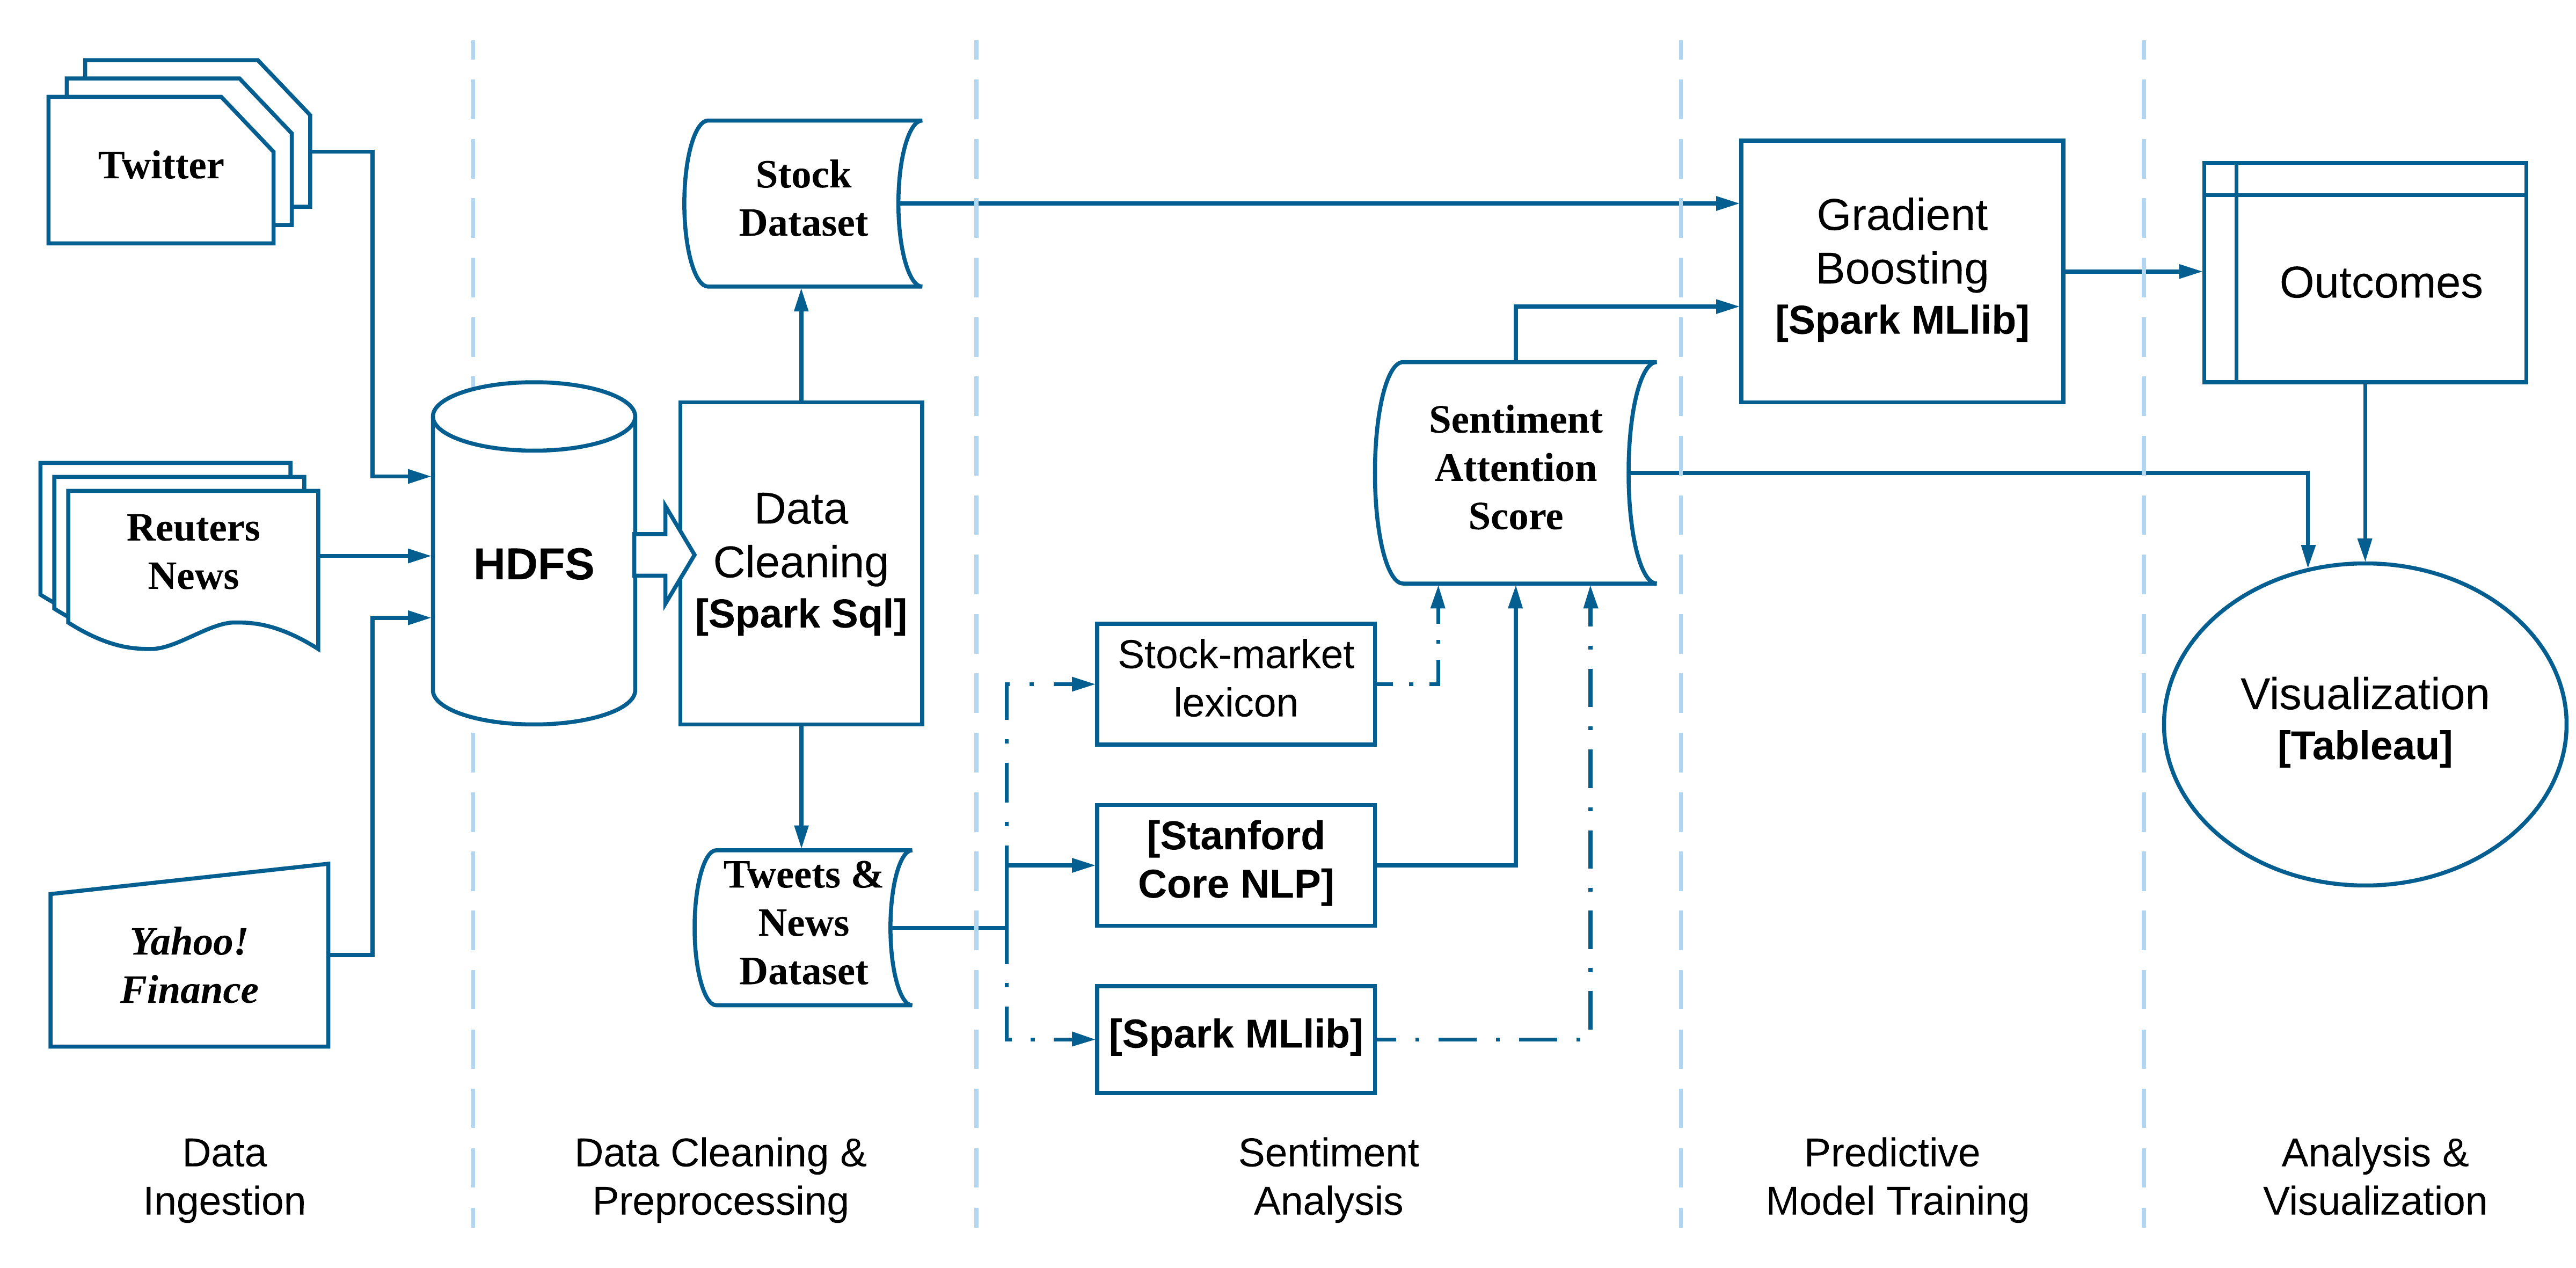
\includegraphics[width=0.9\textwidth]{pics/appdesign.png}
\caption{Design diagram of the investment assistant application}
\label{design}
\end{figure*}

The full design diagram is shown in Figure \ref{design}. The program procedure of our investment assistant application can be divided into five stages.

The first stage is data ingestion. We collect historical data from Twitter, Reuters.com, and Yahoo! Finance and store them on HDFS. The tweets are scrapped by using a Python wrapper over Twitter Standard search. The news headlines on Reuters.com are collected from Reuters News archive. And from Yahoo! Finance, we collected stock price data for more than six thousand stocks listed on NYSE, American Express, and Nasdaq.

Secondly, we perform data cleaning and formatting respectively on each dataset. Each field in each dataset will be explained in Section \ref{Datasets}.

The next stage plays an key role in our application, which is to extract social sentiment and attention scores from tweets and news headings. We have employed three different approaches: 
\begin{itemize}
    \item[i.] by using a stock-market lexicon provided by Oliveira, Paulo, and Nelson\cite{stocklexicon} to assign a sentiment score to each word in the tweet or headline, then compute the mean value as the sentiment score of the tweet or headline;
    \item[ii.] by using language models from Stanford CoreNLP \cite{StanfordNLP} and assign an sentiment score for each tweet or news headline;
    \item[iii.] by training a machine learning model using Spark MLlib on all tweets and news headlines during 2010 to 2015, which is considered as the training set in our application; then use this trained model to predict the sentiment score for each tweet or headline.
\end{itemize}
The attention score is computed as the number of tweets/news related to the stock, normalized by the average number of posts per day in the past month. 

The fourth stage is to identify the relationship between stock excess returns and social sentiment/attention. We use the sentiment score and attention score from previous stage as features. The labels are generated from the stock return, which contains three classes: \textit{Up}, \textit{Down}, and \textit{Fluctuation}. We consider stock price goes up more than 0.85\% as \textit{Up}, and goes down more then 0.85\% as \textit{Down}, all other price movements that less than 0.85\% are considered as \textit{Fluctuations}.

In the end, we present the results of predictive model, which are predictions of the price movements (or investment suggestions) based on the social sentiment and attention. We visualize the trends of social sentiments and stock price using Tableau to help users better understanding their relationships, also we present the statistics of predictive model performance.


\subsection{Visualization Design}
In this assistant application, we present our users with following contents:
\begin{itemize}
    \item[i.] Insights from Twitter: what’s the heated topics on twitter (snapshot at certain time stamp).
    \item[ii.] Mapping the trends on Twitter to Stock Market: investment suggestions generated from predictive model (snapshot at certain time stamp).
    \item[iii.] Tracking the historical performance of each sector of stocks (or other classifications, or specified stocks/stock indices).
    \item[iv.] The performance of our investment strategy.
\end{itemize}

\begin{figure}[H]
\centering
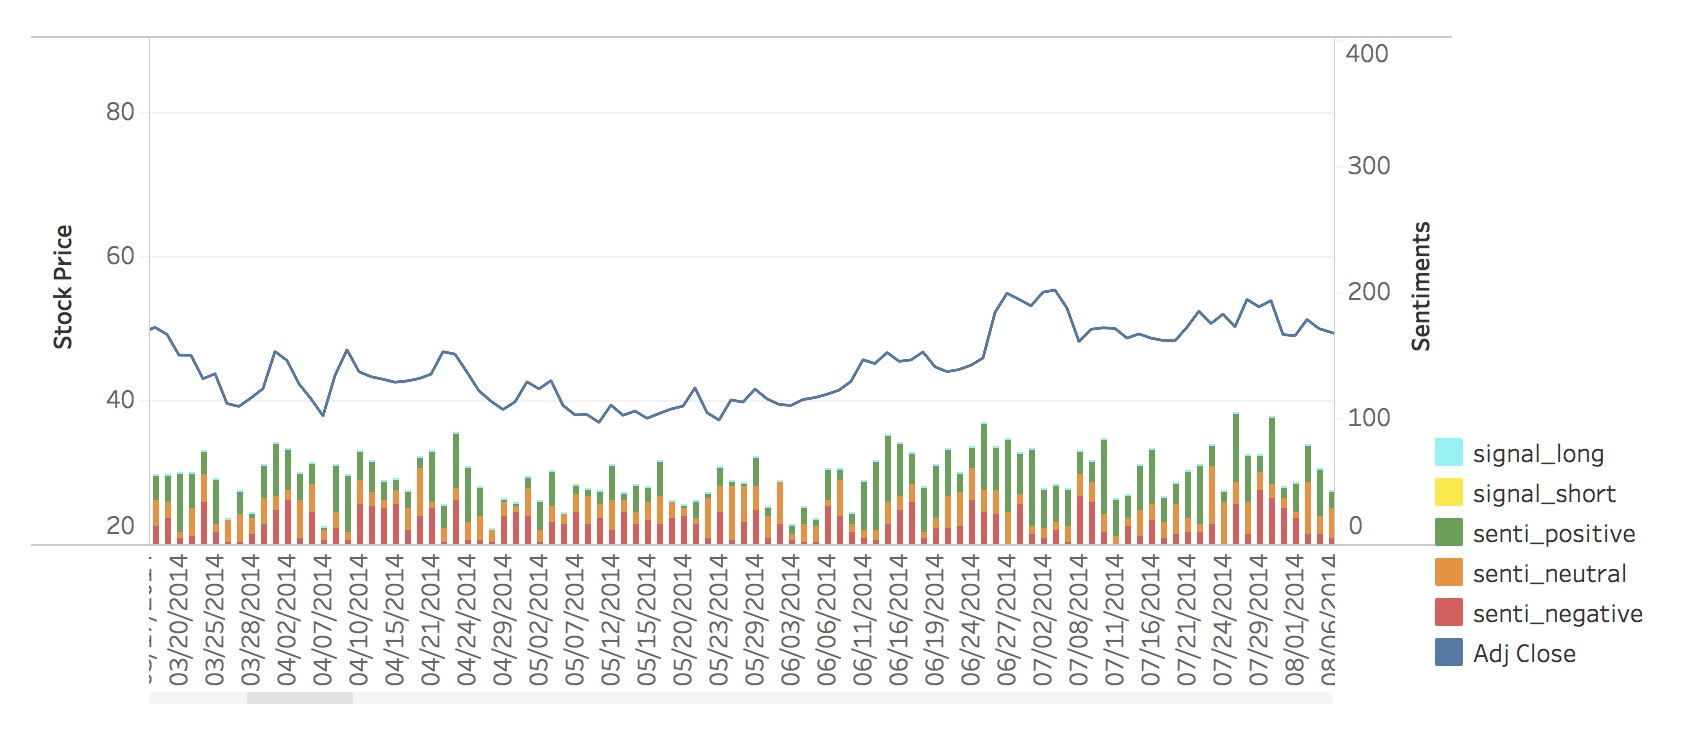
\includegraphics[width=\columnwidth]{pics/visualsample.png}
\caption{An Sample of Visualization Design for Social Sentiment Trending}
\label{visualsample}
\end{figure}
An sample of the visualization is given in Figure \ref{visualsample}. This investment assistant application actually serves as an social sentiment monitor for selected ticker. The sentiment scores for positive, negative and neutral sentiment per day are presented by bars with different color. The full explanation of visualization is given in Section \ref{Experiments}.
\vspace{1.0em}

% --------------------------------------------------------- V. Datasets
\section{Datasets}\label{Datasets}
In order to unify the whole timeline of our final result, all of our historical datasets are collected from January 1st, 2010 to March 31st, 2018.
\vspace{0.5em}

\subsection{Twitter Feeds Dataset}
Our Twitter feeds dataset is consisted of two parts. Firstly, we pulled millions of historical tweets tweeted by famous businessmen and financial news accounts--such as NYSE or Nasdaq--since 2010 from Twitter using a Python library \textit{GetOldTweets} developed by Jefferson Henrique\footnote{https://github.com/Jefferson-Henrique/GetOldTweets-python.}. This part of dataset will be used as a training set in order to analyse each stock or company’s social attention and sentiment index. After that, we kept collecting everyday’s new tweets from individuals as our validation set.

The contents of each collected tweets in our dataset are including:
\begin{itemize}
    \item[a.] \textit{created\_at}: The exact time when this tweet was tweeted.
    \item[b.] \textit{id(id\_str)}: A unique id of this tweet.
    \item[c.] \textit{text}: The main body of this tweet.
    \item[d.] \textit{truncated}: A boolean type variable showing if the tweet is shown completely.
    \item[e.] \textit{lang}: The language used by this tweet. 
    \item[f.] \textit{timestamp\_ms}: The time stamp of this tweet. 
    \item[g.] \textit{reply\_count}: Number of people who replied under this tweet.
    \item[h.] \textit{retweet\_count}: Number of people who retweeted this tweet.
    \item[i.] \textit{favourite\_count}: Number of people who liked this tweet.
    \item[j.] \textit{quote\_count}: Number of people who quoted this tweet.
\end{itemize}
\vspace{0.5em}

\subsection{Reuters News Dataset}
This dataset contains full unofficial data set of Reuters composed of 9,211,932 news titles and timestamps from January 2010 to March 2018, which cover politics, economy, and social communities fields.

All the data were scratched from Reuters archive website, where each day’s Reuters news were collected since 2007. We used a Python library called BeautifulSoup in order to pull out data from HTML pages.

After cleaning the dataset, each line represents a news and is stored in a form as shown below:
\begin{itemize}
    \item[a.] \textit{ts}: The timestamp of this news.
    \item[b.] \textit{title}: The title of this news.
    \item[c.] \textit{herf}: A html link to the main article of this news
\end{itemize}

\subsection{Stock Market Dataset}
We collect the stock prices on each trading day from Yahoo! finance. This dataset is used to calculate daily return of each stock since January 2010 until March 2018, and it will help us drawing relation curve between timestamp, Stock prices and their returns. Through comparing this curve with social attention and social sentiment about certain fields or industries, we are able to conclude an investment advice for our users.

After cleaning the dataset, the contents of each stock in our dataset are including:
\begin{itemize}
    \item[a.] \textit{date}: The day of trading executed.
    \item[b.] \textit{symbol}: Symbol that identify a particular stock.
    \item[c.] \textit{open}: Opening weighted average stock value in USD.
    \item[d.] \textit{close}: Closing weighted average stock value in USD. 
    \item[e.] \textit{high}: All day high in USD.
    \item[f.] \textit{low}: All day low in USD.
    \item[g.] \textit{volume}: Number of trades of this stock.
    \item[h.] \textit{adj close}: Adjusted closing prices (for both dividends and splits) in USD.
\end{itemize}
\vspace{1.0em}

% --------------------------------------------------------- VI. Remediation
\section{Remediations}\label{Remediations}
In the first stage, we present three trend lines: i. historical time series of public sentiment towards the target stock/sector; ii. historical time series of attentions on the target stock/sector; iii. the time series of stock daily return. Experienced investor can utilize these trend lines and make decisions based on the certain patterns. For example, when the sentiment is positive and the objective stock gets considerable attention, and the price is below the historical mean, then investors can feel free to take long positions.

One step further, we provide our own trading strategies based on the relations of the above trend lines. We evaluate the portfolio returns (a portfolio is a set of stocks selected by a certain strategy) with respect to interest free rate. If our portfolio outperforms interest free rate, it implies the insights extracted from news media really works in practical.
\vspace{1.0em}

% --------------------------------------------------------- VII. Experiments
\section{Experiments}\label{Experiments}
\begin{figure}[t]
\centerline{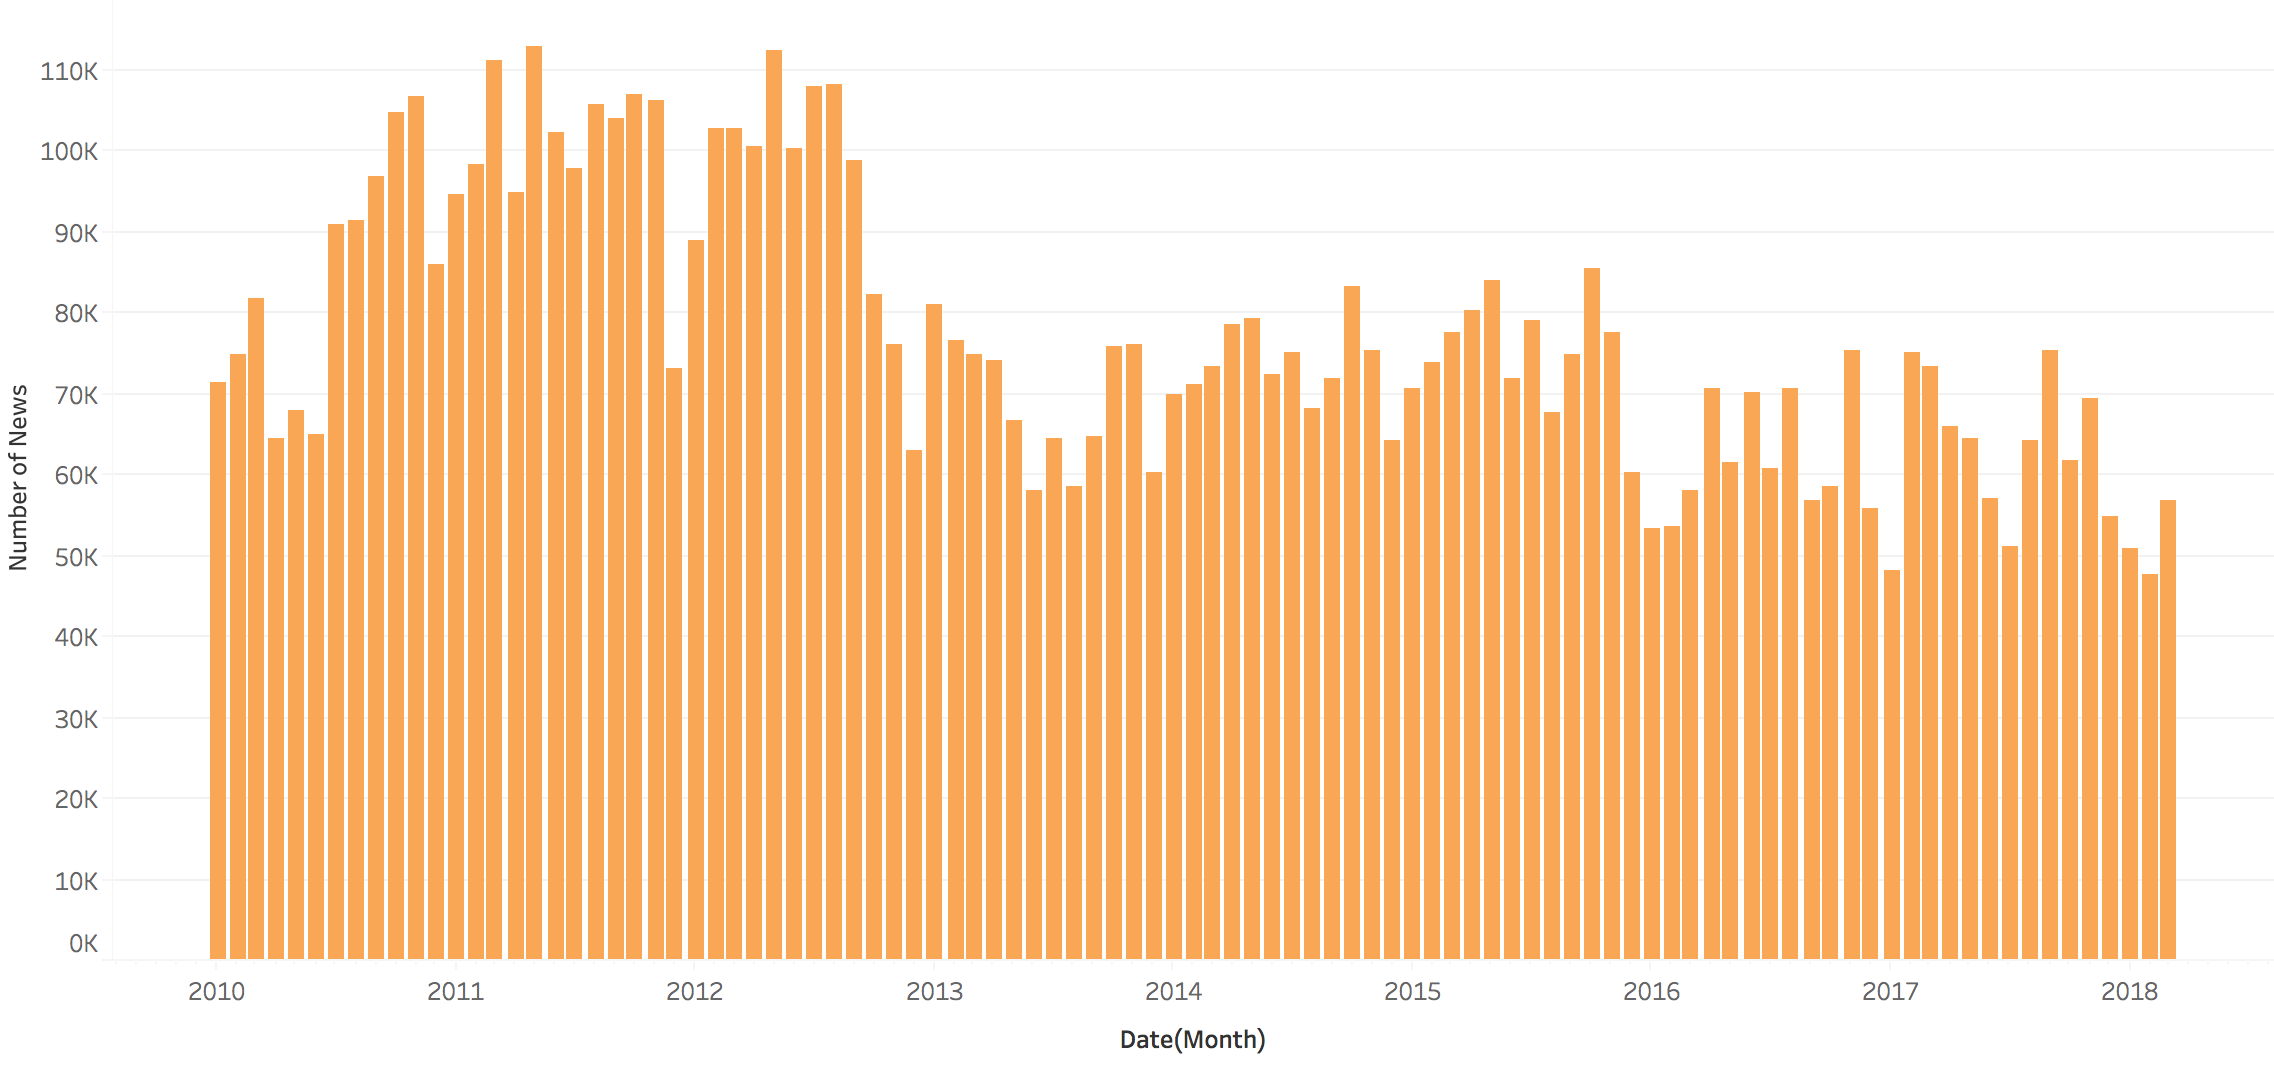
\includegraphics[width=\columnwidth]{pics/reutersImage.png}}
\caption{Daily post count of news on Reuter.com}
\label{reuters}
\end{figure}

\begin{figure}[t]
\centerline{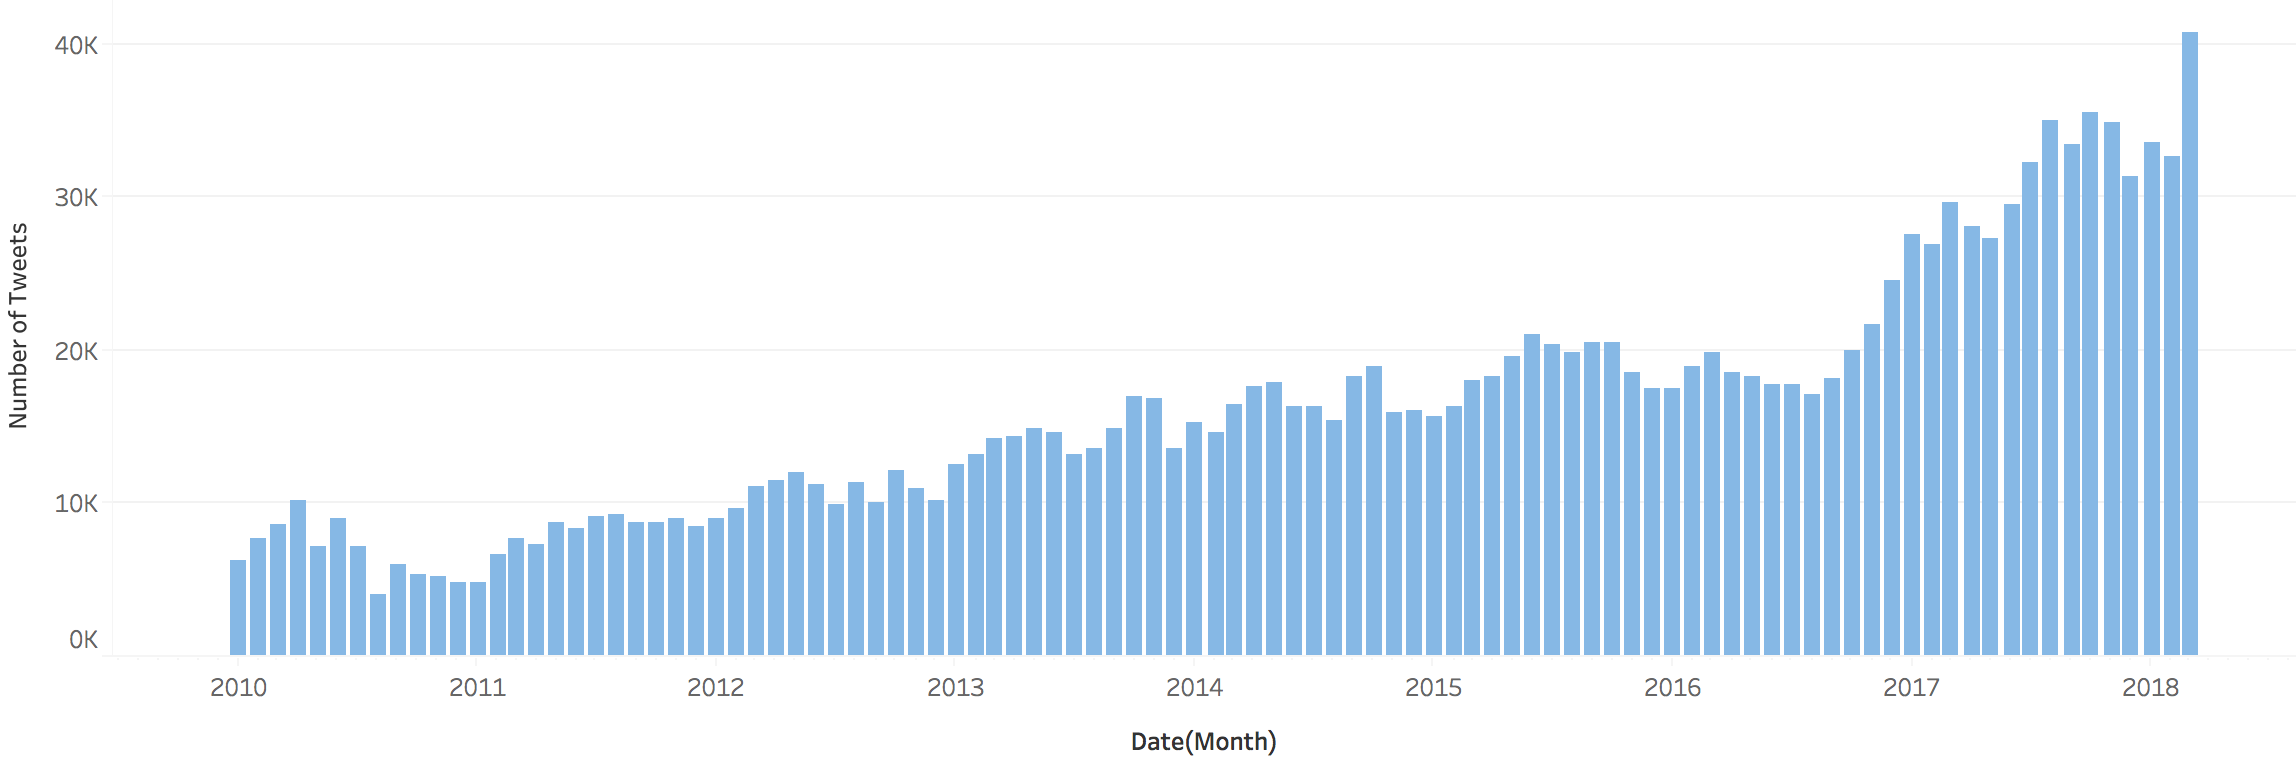
\includegraphics[width=\columnwidth]{pics/twitterImage.png}}
\caption{Daily post count of tweets in collected dataset}
\label{twitter}
\end{figure}


First, we present an overview of the social media data. The daily count of tweets that we have collected is shown in Figure \ref{twitter}. And the general posting daily count of news on Reuters.com is shown in Figure \ref{reuters}. There are 10 sectors in the stock market, including Consumer Staples, Consumer Discretionary, Energy, Financial, Health Care Services, Industrial, Information Technologies, Materials, Telecommunication Services, and Utilities. The distribution of social attention from tweets and news are shown in Figure \ref{sectorNews} and Figure \ref{sectorTwitter} respectively. 

\begin{figure}[t]
\centerline{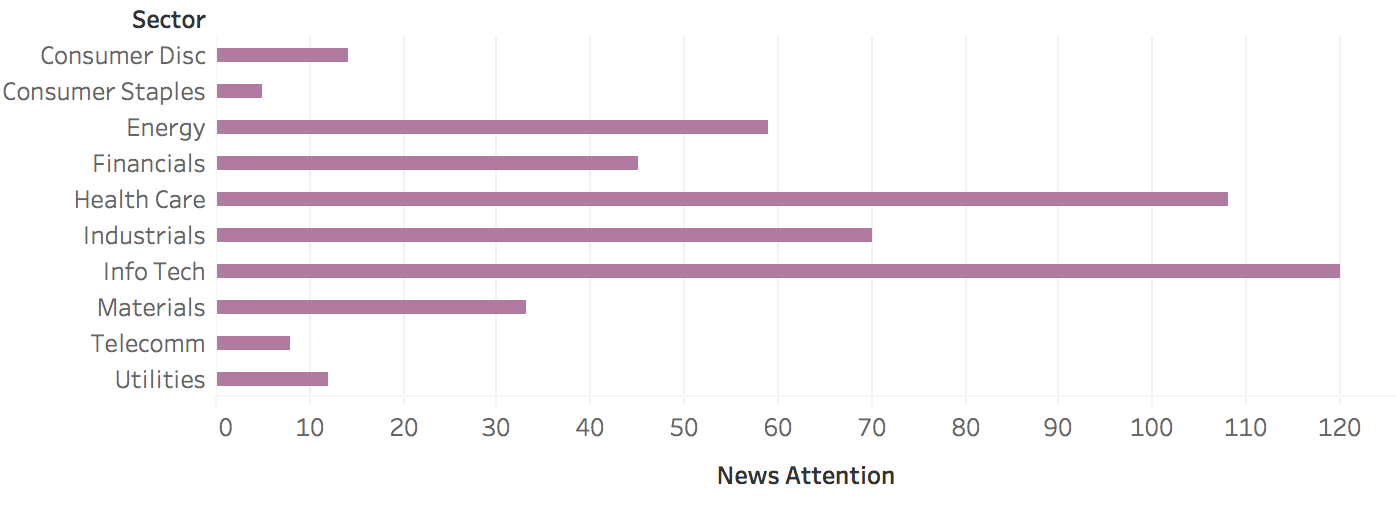
\includegraphics[width=\columnwidth]{pics/newsAttention.png}}
\caption{Social attention from Reuters News distribution among 10 sectors.}
\label{sectorNews}
\end{figure}

\begin{figure}[t]
\centerline{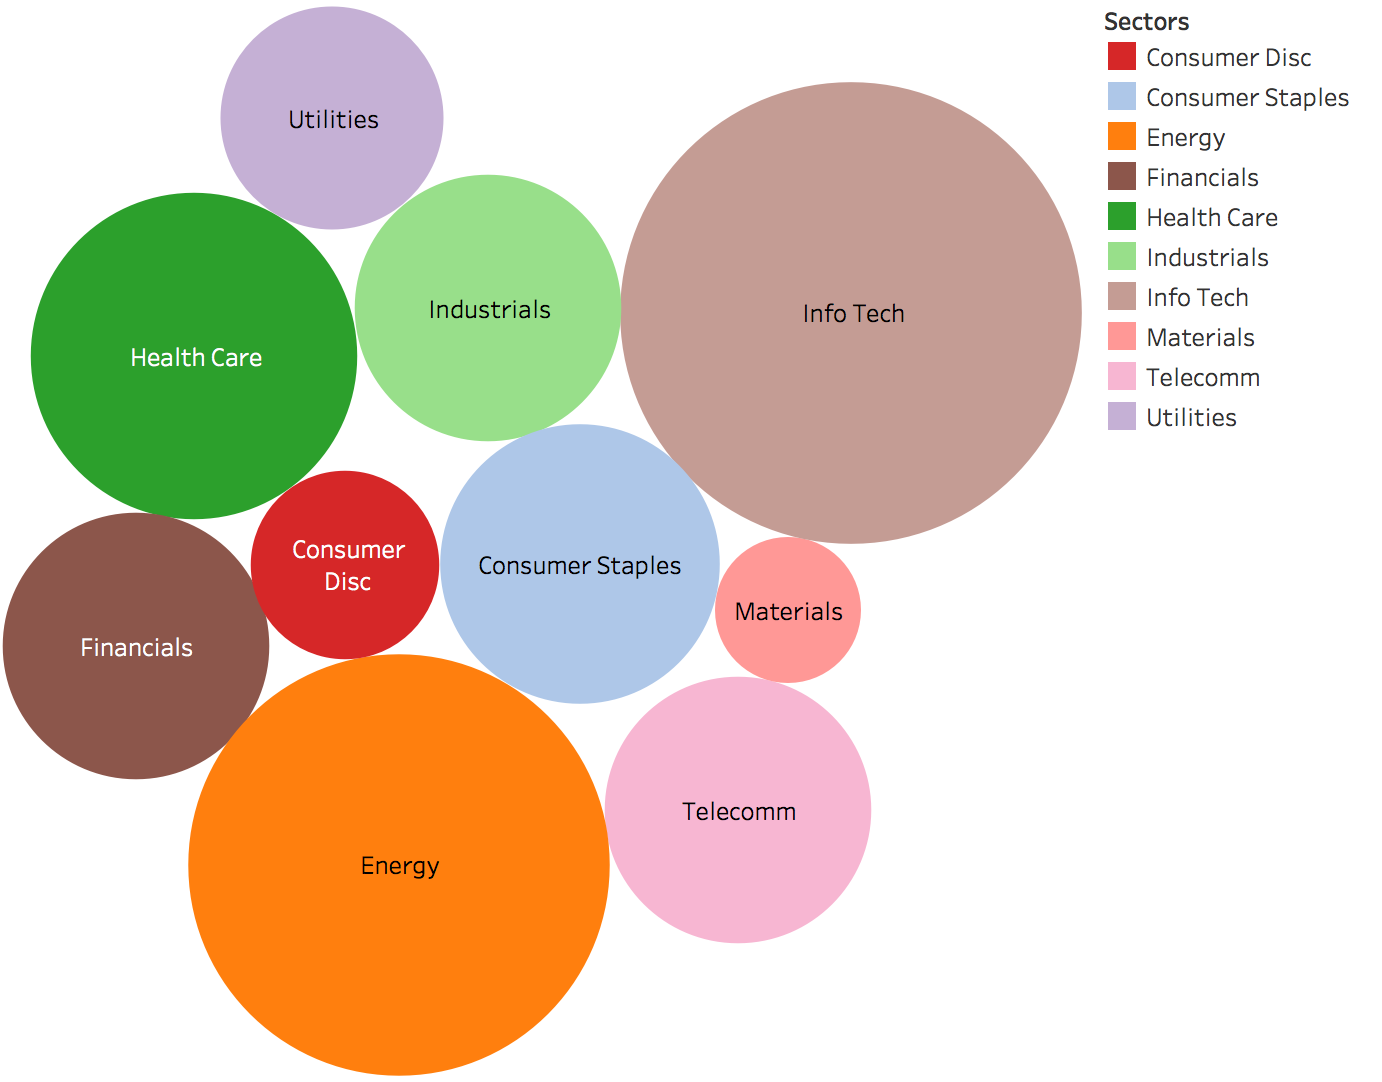
\includegraphics[width=0.8\columnwidth]{pics/sectorImage.png}}
\caption{Social attention on Twitter distribution among 10 sectors.}
\label{sectorTwitter}
\end{figure}

As a demonstration of social sentiment visualization for selected ticker, we provide the visualization result for ticker WUBA in Figure \ref{wuba}. The company, 58.com Inc., operates online classifieds and listing platforms that enable local merchants and consumers to connect, share information, and conduct business in China.

To help readers have a clear view of the sentiment visualization, we select the time period from March 3rd, 2015 to December 30th, 2015. The sentiment scores for positive, negative and neutral sentiments are shown in green, red and orange respectively. Besides, there are long/short signals generated from the social sentiments and attention (attention can be visualized from the height of the bar each day). A long signal indicates that the stock price is about to go up, and short signal for price down. 

In order to evaluate the predictive performance of our sentiment alert signals, we train a 3-class classifier by using sentiment and attention scores as features, and stock price up-and-downs as labels. As mentioned in Section \ref{Design}, the price movement is categorized into 3 classes: \textit{Up}, \textit{Down} and \textit{Fluctuation}. The train-validation-split is done by using 2010 to 2015 as training set, and 2016 to 2017 as validation set. We do not use the first three month of 2018 in validation set, because we need three more months of stock price data to compute the return of next one quarter at the end of 2017. 

\begin{figure*}[ht]
\centering
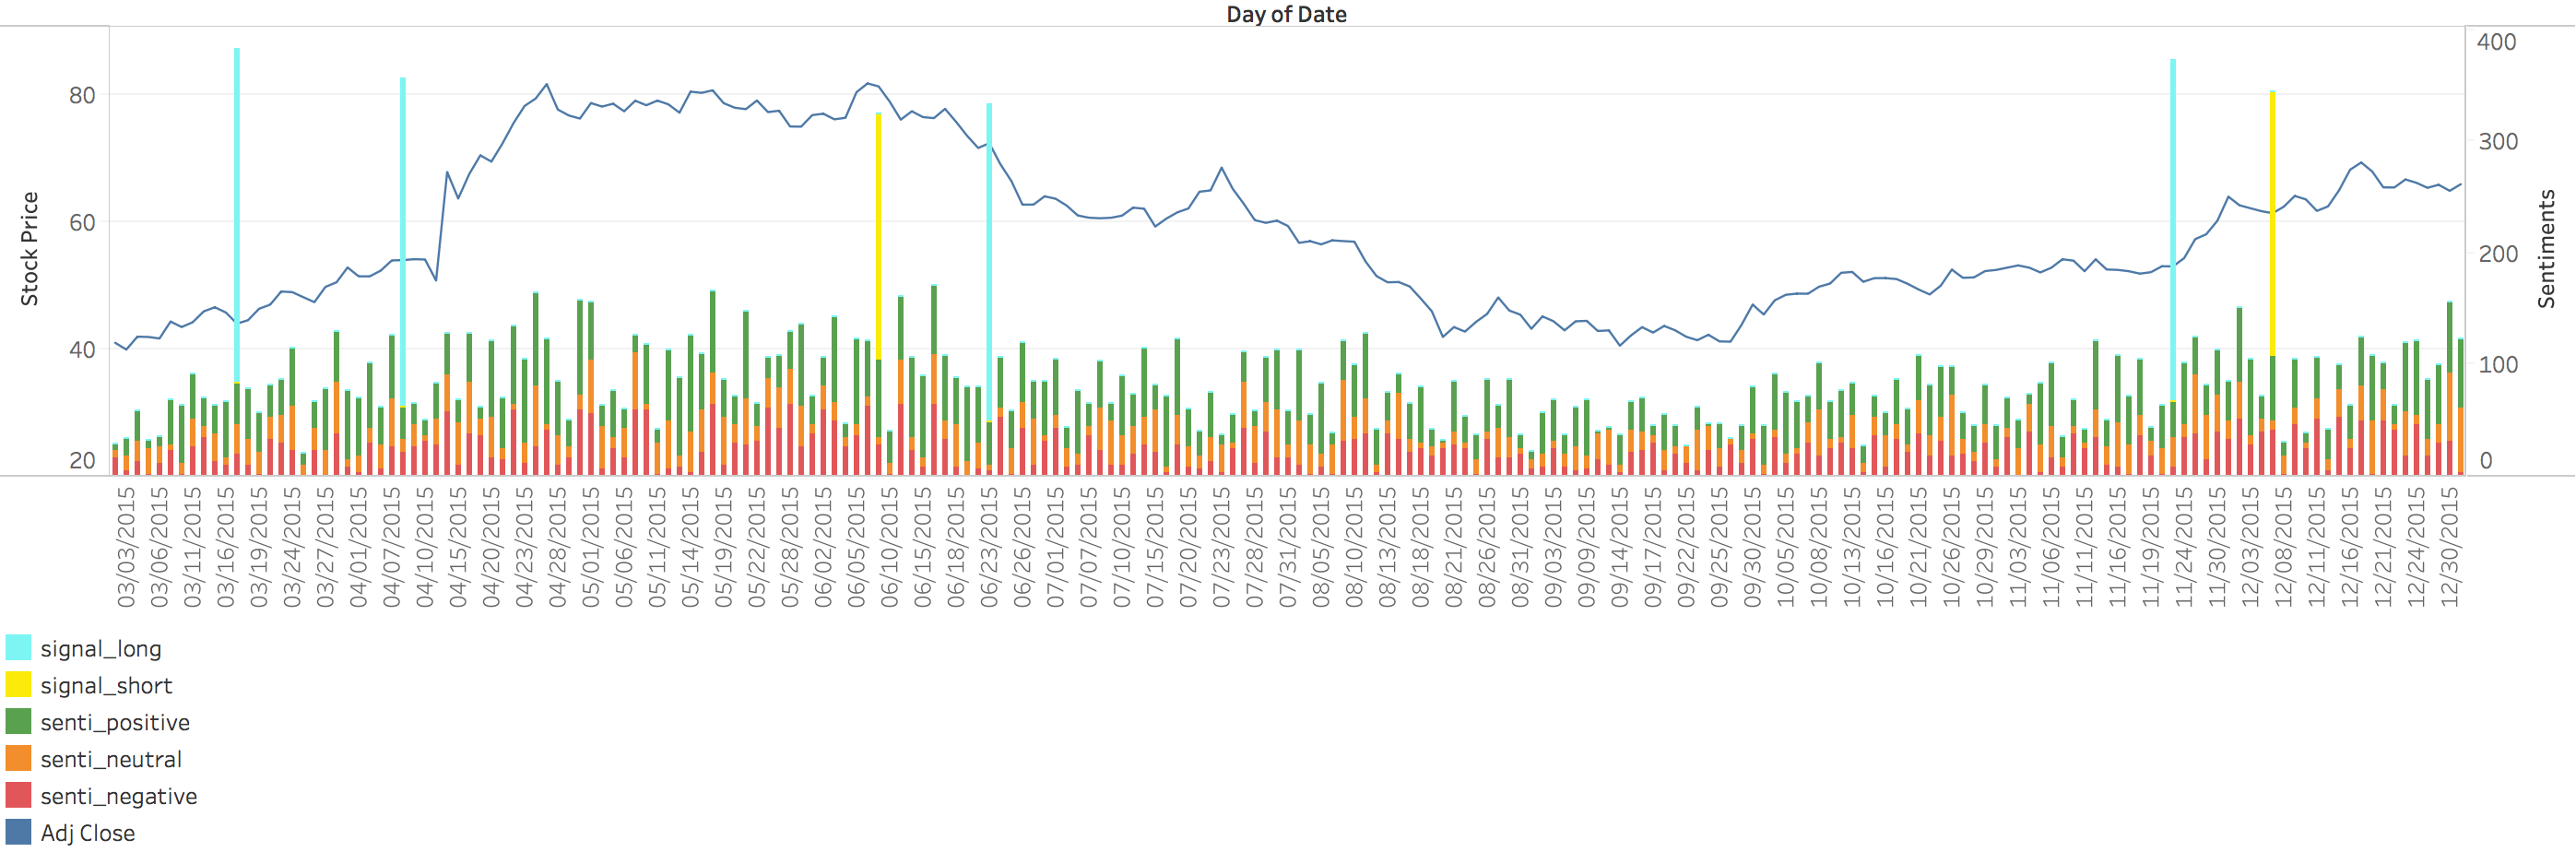
\includegraphics[width=0.9\textwidth]{pics/wubaNew2.png}
\caption{Demonstration of sentiment alert signals on ticker \$WUBA }
\label{wuba}
\end{figure*}

We have employed three NLP methods to extract sentiment score, and train an classifier using Gradient Boosting algorithm on the result from each of them. The performance of classification accuracy is presented in Table \ref{accuracytable}. We can see that the Stanford CoreNLP outperforms the others. It is likely that the complex language model embedded in Stanford CoreNLP helps with understanding the sentiments in tweets and news headlines. 

\begin{table}[bp]
\caption{Prediction accuracy using different NLP approaches to extract social sentiment}
\begin{center}
\begin{tabular}{|c|c|c|}
\hline
\textbf{Accuracy} & \textbf{\textit{Training}}(2010-2015)& \textbf{\textit{Validation}}(2016-2017) \\
\hline
Gradient Boosting & 72.52 & 67.92  \\
\hline
Stock market lexicon & 75.66 & 76.31  \\
\hline
Stanford CoreNLP & 83.30 & 77.72  \\
\hline
\end{tabular}
\label{accuracytable}
\end{center}
\end{table}

\begin{figure}[tb]
\centerline{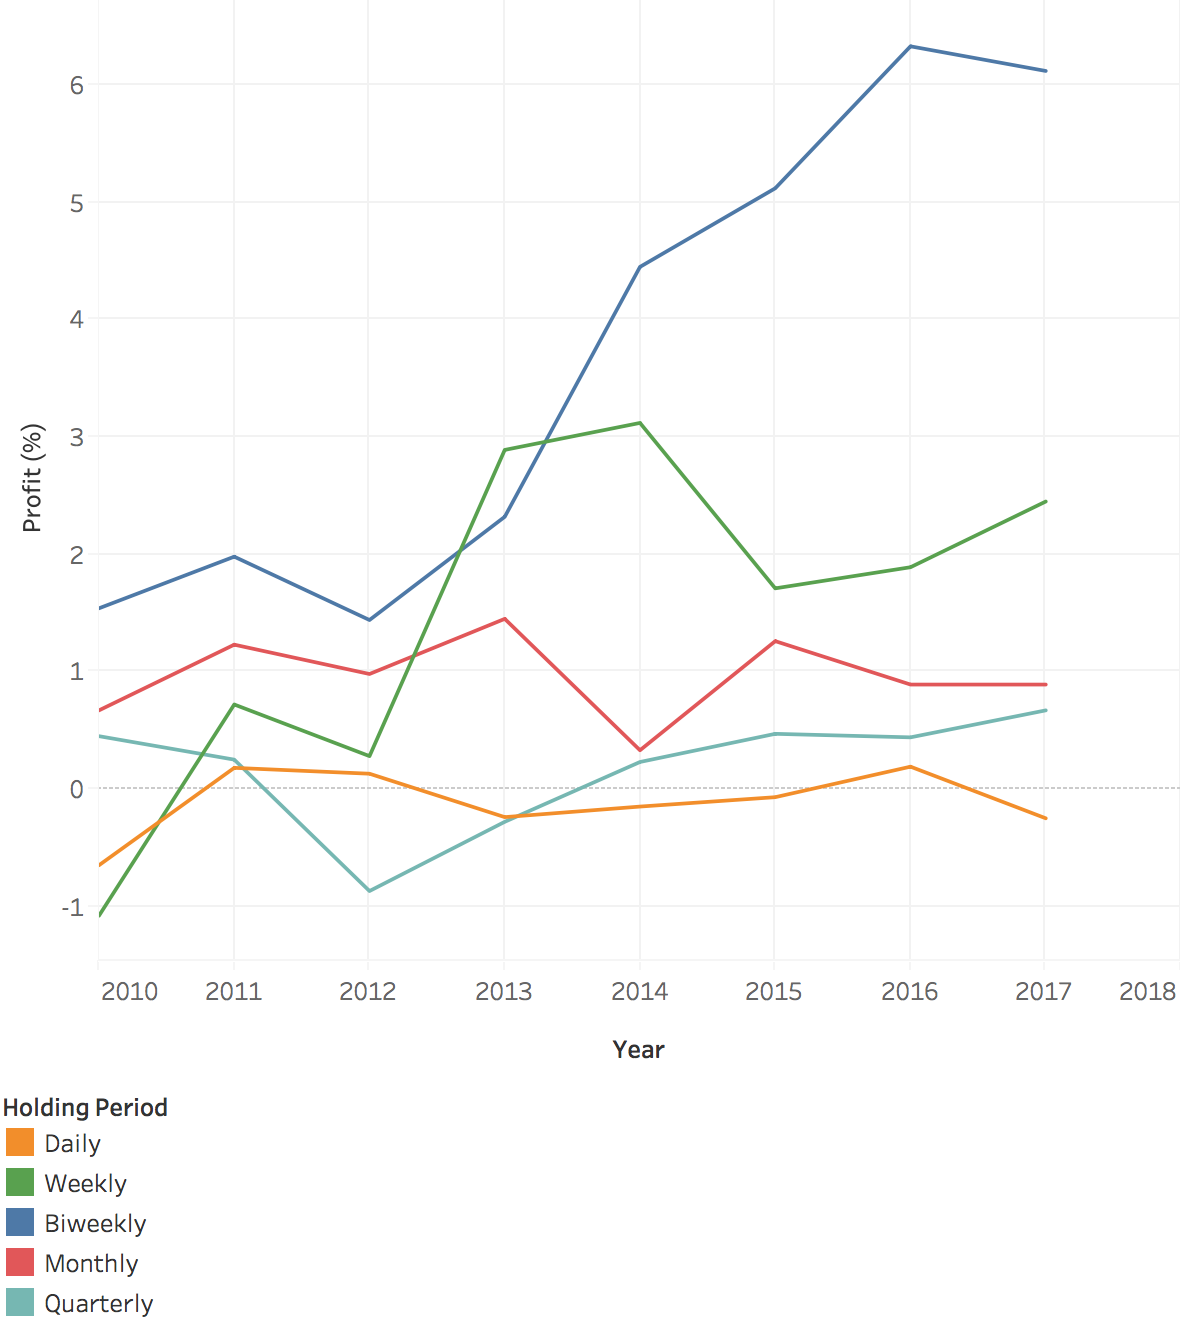
\includegraphics[width=0.9\columnwidth]{pics/annualprofit.png}}
\caption{Average portfolio return based on different holding period after sentiment alert signals}
\label{profitfigure}
\end{figure}

\begin{table}[tb]
\caption{Average Portfolio return based on different holding period after sentiment alert signals (2010-2017)}
\begin{center}
\begin{tabular}{|c|c|c|c|c|c|}
\hline
\textbf{Hold-days} & \textbf{\textit{1 Day}}& \textbf{\textit{5 Days}}& \textbf{\textit{10 Days}} & \textbf{\textit{21 Days}} & \textbf{\textit{63 Days}} \\
\hline
Return(\%) & -0.12 & 1.53 & \textbf{3.66} & 0.96 & 0.17 \\
\hline
\end{tabular}
\label{profit}
\end{center}
\end{table}

The prediction accuracy is not our objective. Our users are more concerned about the profit it brings. So we performs the following experiments to evaluate the profitability of our sentiment alert signals. We construct portfolios with corresponding stocks with long/short signals. There are 1187 stocks that meet the minimum social attention requirement for trading on social sentiment. And we trade the stock if a long/short signal is generated based on the sentiments of last 5 trading days (one week in practical). Then we compute the stock return in the next N days, N = 1, 5, 10, 21, 63. The annual average profit of each trading strategy is shown in Figure \ref{profitfigure}. And the average return rates for each transaction based on the trading strategies are listed in Table \ref{profit}.

Considering Table \ref{profit} and Figure \ref{profitfigure}, it brings the most profit when we close the positions in two weeks after opening. And this phenomenon becomes more promising in recent years: it achieves an average return rate of 5.52\% in 2014-2017. 
\vspace{1.0em}

% --------------------------------------------------------- VIII. Conclusion
\section{Conclusion}\label{Conclusion}
Social signals provide another tool for investors to identify trends and events that may move or influence markets.

We have shown that social sentiment and attention can provide predictive information about stock price. Such prediction has high accuracy and performs consistent over time. 

By using our application, we are able to capture current and potential price movements ahead of the market, in the form of sentiment alert signal. As shown in our analysis, the market actually takes two weeks to absorb and digest the information of public mood. Users could use their own judgment to make investment decisions based on the sentiment alert signals, or use the trading strategies provided by the application. Our investment assistant application can benefit us and our customers take favorable positions in financial market. 

In the future, we would develop real-time social sentiment processing by using Spark Streaming, which would make our application a investment assistant in real world trading. 
\vspace{1.0em}

\section*{Acknowledgment}

We appreciate the previous works from research teams of Stanford Core-NLP providing the natural language software, and team of Cloudera Data Science team for the spark-ts library. We also give our appreciations to Oliveira research team for their contribution on the lexicon targeting at stock market. 
And we sincerely appreciate Prof. Suzanne McIntosh and NYU HPC for their support with Spark application development. 

%\section*{References}

\begin{thebibliography}{00}
\bibitem{Kim} Y. Kim, S. Ryul Jeong, and I. Ghan.i. Text Opinion Mining to Analyze News for Stock Market Prediction. Int. J. Advance. Soft Comput. Appl., Vol. 6, No. 1, March 2014 ISSN 2074-8523
\bibitem{Oliveira} N. Oliveira, P. Cortez, and N. Areal. The impact of microblogging data for stock market prediction: using Twitter to predict returns, volatility, trading volume and survey sentiment indices. Expert Syst. Appl., 73 (2017), pp. 125-144
\bibitem{Zhang} W. Zhang and S. Skiena, Trading Strategies to Exploit Blog and News Sentiment. In Proceedings of the International Conference on Weblogs and Social Media, 2010.
\bibitem{Pagolu} V. S. Pagolu, K. N. R. Challa, G. Panda, and B. Majhi, “Sentiment analysis of Twitter data for predicting stock market movements,” in Proceedings of the International Conference on Signal Processing, Communication, Power and Embedded System (SCOPES 2016), 2016, p. 6. [Online]. Available: http://arxiv.org/abs/1610.09225
\bibitem{Mao} Mao Y, Wei W, Wang B, Liu B. Correlating S\&P 500 stocks with Twitter data. In: Proc. 1st ACM Intl. Workshop on Hot Topics on Interdisciplinary Social Networks Research; 2012. p. 69–72.
\bibitem{Ruiz} Ruiz, E. J., Hristidis, V., Castillo, C., Gionis, A. and Jaimes, A. 2012. Correlating financial time series with micro-blogging activity. In Proceedings of the fifth ACM international conference on Web search and data mining (WSDM-2012), 513-522.
\bibitem{Ranco} Ranco, G., Aleksovski, D., Caldarelli, G., Grčar, M., and Mozetič, I. (2015). The effects of twitter sentiment on stock price returns. PloS One, 10(9). e0138441
\bibitem{Lekha} Lekha R. Nair and DR. Sujala D. Shetty, Streaming Twitter Data Analysis Using Spark For Effective Job Search. In Journal of Theoretical and Applied Information Technology,. Vol.80. No. 2 2005 – 2015.
\bibitem{Kouloumpis} Kouloumpis, E., Wilson, T., Moore, J.: Twitter Sentiment Analysis: The Good the Bad and the OMG! In: Proceedings of the ICWSM (2011)
\bibitem{Kireyev} K. Kireyev, L. Palen, and K. M. Anderson. Applications of Topics Models to Analysis of Disaster-Related Twitter Data. NIPS Workshop on Applications for Topic Models: Text and Beyond (2009)
\bibitem{Corvey} W. J. Corvey, S. Vieweg, T. Rood and M. Palmer. Twitter in Mass Emergency: What NLP Techniques Can Contribute. WSA '10 Proceedings of the NAACL HLT 2010 Workshop on Computational Linguistics in a World of Social Media, Pages 23-24.
\bibitem{Chae} Bongsug (Kevin) Chae. Insights from hashtag \#supplychain and Twitter Analytics: Considering Twitter and Twitter data for supply chain practice and research. Int. J. Production Economics 165 (2015) 247–259.
\bibitem{Qi} W. Qi, L. Gu, H. Jiang, X. Chen and H. Zhang.Integrating visual, audio and text analysis for news video. 2000 International Conference on Image Processing (Cat. No.00CH37101)
\bibitem{stocklexicon}Oliveira, Nuno, Paulo Cortez, and Nelson Areal. Stock market sentiment lexicon acquisition using microblogging data and statistical measures. Decision Support Systems 85 (2016): 62-73.
\bibitem{StanfordNLP} Manning, Christopher D., Surdeanu, Mihai, Bauer, John, Finkel, Jenny, Bethard, Steven J., and McClosky, David. 2014. The Stanford CoreNLP Natural Language Processing Toolkit In Proceedings of 52nd Annual Meeting of the Association for Computational Linguistics: System Demonstrations, pp. 55-60.

\end{thebibliography}


\end{document}
